\documentclass[a4paper, 1.5lines]{ctexart}
\usepackage[top=3cm, bottom=2cm]{geometry}
\usepackage{graphicx}
\usepackage{subcaption}
\usepackage{amsmath}
\usepackage{xcolor}
\usepackage{url}
\usepackage{booktabs}
\usepackage{multirow}
%\usepackage{hyperref}
\usepackage[hidelinks]{hyperref} % 加载 hyperref 并隐藏链接边框

%\usepackage[utf8]{inputenc}
%\usepackage[ngerman]{babel} % 加载德语支持

% booktabs 提供 \toprule, \midrule, \bottomrule 等表格命令
\usepackage{booktabs}
% 定义占位命令以避免未定义控制序列错误
\newcommand{\placeholderspace}{}
\usepackage{fancyhdr} % 导入fancyhdr宏包
\usepackage{lipsum}   % 仅用于生成示例文本
\usepackage{float}    % 提供 H 浮动位置选项

% 设置页面样式为fancy
\pagestyle{fancy}
% 自定义页眉内容
\fancyhead[L]{} % 左侧页眉
\fancyhead[C]{\textbf{Physics-experiment Reporting Letter:\\Nonlinear Circuit’s Chaos and Its Application}} % 中间页眉
\fancyhead[R]{ } % 右侧页眉
% 自定义页脚内容
\fancyfoot[L]{ } % 左侧页脚
\fancyfoot[C]{\thepage} % 中间页脚显示页码
\fancyfoot[R]{ } % 右侧页脚
% 改变页眉线的粗细
\renewcommand{\headrulewidth}{1.4pt}
% 改变页脚线的粗细
\renewcommand{\footrulewidth}{0.pt}





\title{非线性电路}
\author{实验人：唐亿\qquad 学号：202311998381\qquad 指导教师：张金星}
\date{实验日期：2025.10.24}


\begin{document}
    
    \maketitle
    
    \begin{abstract}
         混沌不仅是是非线性动力学系统的本质属性，也是混沌同步与通信的理论基础。这一特征可以在简单的蔡氏电路中通过倍周期分岔得到实现。本实验测量了蔡氏电路核心元件非线性负阻的$ I-U $特性曲线，并进一步研究了蔡氏电路中两电容提供的相图的动态变化，以此得到了倍周期分岔通向混沌的一系列状态，并借助电容箱对分岔参量进行测量，估计了准费根鲍姆常数。此外，实验还实现了两个蔡氏电路的混沌同步，观察了从同步到去同步的变化过程，并在此基础之上实现了混沌加密通信。
    \end{abstract}
    
    \section{引言}
       19世纪末20世纪初，法国数学家庞加莱在解决天体力学中的三体问题时，把动力学系统和拓扑学有机地结合起来，提出了庞加莱猜想，此外他指出三体问题的解在一定范围内是随机的，非线性科学的思想萌芽。1963年，美国气象学家洛伦茨（Lorenz）在《确定论的非周期流》一文中，给出了描述大气湍流的洛伦茨方程，并提出著名的“蝴蝶效应”，揭开了对非线性科学深入研究的序幕，非线性科学得以真正建立。1990年Pecora和Carroll提出了实现混沌同步的驱动——响应方法，混沌同步理论的研究及其在保密通信中的应用成为了一个新的研究热点。
    
        由于电路元器件具有可以被精确控制的特点，非线性振荡电路可以呈现出丰富的混沌现象。蔡氏电路是美国加州大学伯克利分校的华裔科学家蔡少棠设计的能产生混沌行为的最简单的电路，它可以实现倍周期分岔到混沌、再到周期窗口的完整过程，非线性电阻则是该电路的核心器件。本实验将测量非线性负阻的I-U特性曲线，并借助蔡氏电路实现倍周期分岔通向混沌、混沌同步和混沌加密通信等实验，以此加深对于混沌现象及其特征的理解。

    \section{原理}
        本实验借助蔡氏电路产生混沌行为，它由一个非线性电阻$R_N$、电感$L$、可调电阻$R$以及电容器$C_1$和$C_2$组成，其中非线性电阻$R_N$是电路的核心器件。电感器$L$和电容器$C_2$组成一个LC振荡电路；电阻$R$和电容器$C_1$串联将振荡器产生的正弦信号移相输出；$R_N$有两个作用，一是电路的损耗电阻$R$被抵消，使得输出电流维持LC振荡器等幅振荡，另一个作用是使振荡周期产生分岔和混沌等一系列非线性现象。蔡氏电路的电路图如图1所示。
        \begin{figure}
            \centering    
            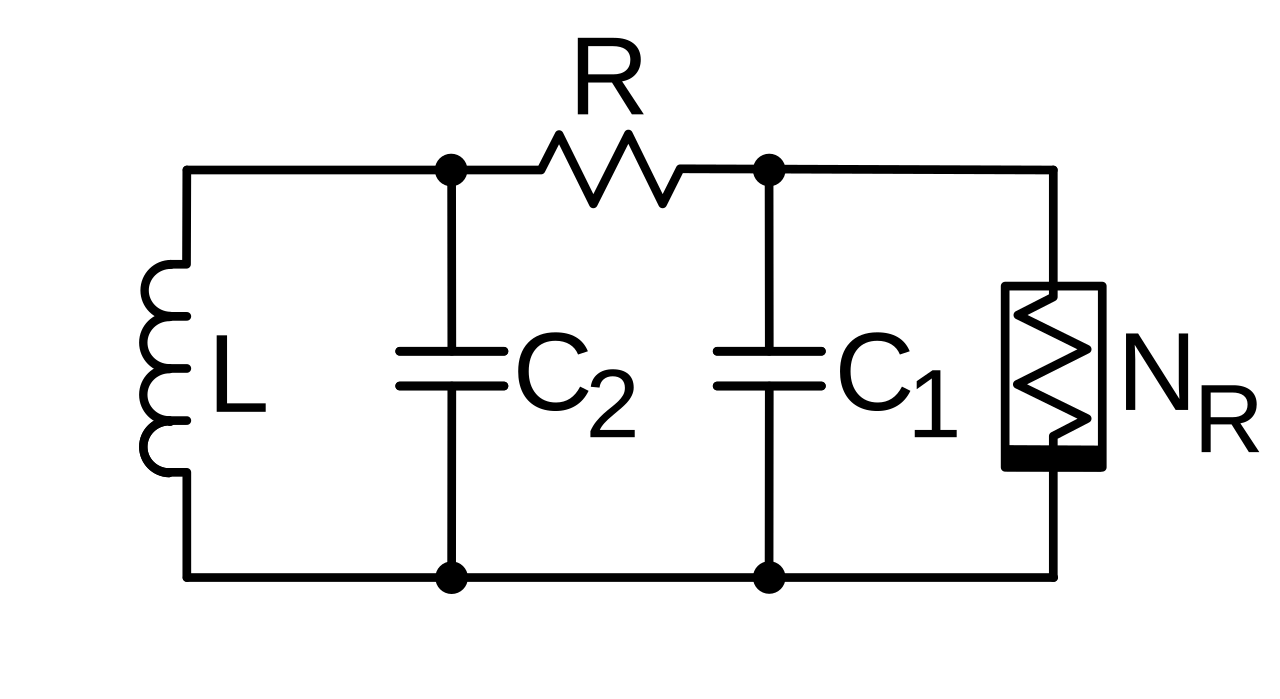
\includegraphics[width=0.8\textwidth]{fig//Chua's_circuit_with_Chua_diode.svg.png} 
            \caption{蔡氏电路示意图}
            \label{fig:RT_curve_experiment}
        \end{figure}
    
    
    \subsection{动力学方程}
    
    电路的动力学方程由基尔霍夫定律给出：
    
    \begin{equation}
        \begin{cases}
            i_{C_1} & = i_{R} - i_{R_N} \\
            i_{C_2} & = i_L - i_R \\
            L\dfrac{\mathrm{d}i_L}{\mathrm{d}t} & = - U_{C_2}
        \end{cases}
    \end{equation}
    从而
    \begin{equation}
        \begin{cases}
            C_1 \dfrac{\mathrm{d} U_{C_1}}{\mathrm{d} t} & = \dfrac{1}{R}(U_{C_2} - U_{C_1}) - \dfrac{1}{R_N(U_{C_1})} U_{C_1}\\
            C_2 \dfrac{\mathrm{d} U_{C_2}}{\mathrm{d} t} & = \dfrac{1}{R}(U_{C_1} - U_{C_2}) + i_L\\ 
            L \dfrac{\mathrm{d} i_L}{\mathrm{d} t} & = - U_{C_2}
        \end{cases}
    \end{equation}
    
    其中$R_N$是非线性负阻，它对$U_{C{\tiny 1}}(=U_{R{\tiny N}})$的依赖性即为电路非线性的体现。
    
    
    \subsection{非线性负阻结构}
    
    本实验用到的有源非线性负阻$R_N$的内部结构如2所示，在给定电路参数下$R_N$的 I-U 特性曲线并不是通常情况下的直线，在某些范围内可能出现电压与电流极性相反的现象，这就是负阻效应。
    
    $R_N$在电路中有两个作用，一是抵消电路的损耗电阻$R$，使输出电流维持LC振荡器等幅振荡；另一个是产生分岔和混沌。$R_N$中同时存在正反馈和负反馈，正反馈的强弱与$R_3/R$和$R_6/R$有关，负反馈的强弱与$R_2/R_1$和$R_5/R_4$有关，当正反馈大于负反馈时，电路才能发生振荡，正反馈的改变可以通过调节$R$来实现。
    
        \begin{figure}
            \centering    
            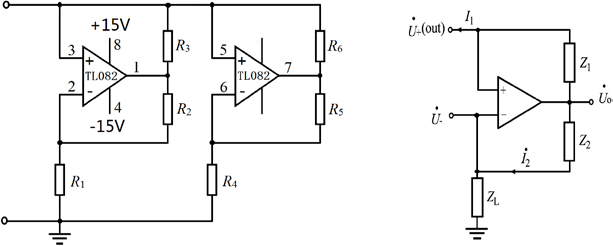
\includegraphics[width=0.8\textwidth]{fig//RN.jpg} 
            \caption{非线性负阻示意图}
        \end{figure}

    \subsection{倍周期分岔通向混沌}
    
    倍周期分岔过程中，系统的振荡周期由P变为2P、继而为$2^2$P、\dots、$2^n$P($n=0,1,2,\dots$)直至出现混沌。该过程中动力学系统的分岔点处参量$\mu$的取值$\mu_n$存在普适规律——相邻参量的比值收敛到一个常数：
    \begin{equation}
        \delta \equiv \lim_{n\to\infty}\delta_n = \lim_{n\to\infty} = \dfrac{\mu_n - \mu_{n-1}}{\mu_{n+1}-\mu_n} = 4.69920\dots
    \end{equation}
    $\delta$称为费根鲍姆常数，任何一个混沌系统都存在着常数$\delta$。实验上通常测量前三个倍周期分岔的参数值来估计费根鲍姆常数。
    
    
    
    \subsection{混沌同步}
    
    混沌同步是指一个系统的混沌动力学轨道收敛于另一个系统的混沌动力学轨道，以致在以后的时间里两个系统始终保持步调一致。通常利用“驱动——响应方法”实现混沌同步——将系统分成驱动子系统和响应子系统，用驱动子系统产生的信号驱动复制的响应子系统。实验中的混沌同步系统由两个相同的蔡氏电路和一个单向耦合系统构成，电路图如图所示，单向耦合系统使得驱动系统只对响应系统产生作用，而响应系统不能对驱动系统作用，从而$R_C$的左右两端便分别为驱动系统的$C_1$信号和响应系统的$C_1^\prime$信号，通过调节$R_C$的大小可以实现两信号的相等。该信息体现于$U_{C1}\sim U_{C1^\prime}$的李萨如图特征。
    
    
    \subsection{混沌通信}
    
    混沌通信是将传输信号混入混沌信号中进行传输，接收方通过（利用混沌同步的原理）减去与之同步的另一混沌信号，即可获得传输信号。混沌通信电路图如图所示，其具体的实现方法如下：
    
    调节驱动系统和响应系统的可变电阻$R$，使它们都出现混沌状态；调节单向耦合电阻$R_C$，使驱动和响应系统同步；$S(t)$是要传输的信号，通过加法器与驱动系统$C_2$的电压混沌信号混合后进行传输，在接收端用减法器将传输信号与响应系统$C_2 ^\prime$的电压混沌信号相减。由于响应系统与驱动系统同步，即$C_2 ^\prime$上的电压信号等于$C_2$上的电压信号，故相减的结果为所需的信号$S^\prime(t)$。由于噪声的影响和电路损耗，$S^\prime(t)$与$S(t)$不完全相同，可以在减法器后接一个滤波器，尽量减小$S^\prime(t)$的噪声。

    \section{实验}
     
        \subsection{实验仪器}
            \subsubsection{蔡氏电路}
                包括电路板、导线、非线性负阻$R_N$、电感$L$、可调电阻$R$以及电容器$C_1$和$C_2$。
            \subsubsection{示波器}
                用于观察电路输出信号的波形和频率。
            \subsubsection{信号发生器}
                提供初始激励信号以启动电路振荡。
            \subsubsection{可变电阻箱}
                用于调节电路中的电阻值，以实现不同的动力学行为。
            \subsubsection{加法器、减法器和滤波器}
                用于混沌通信实验中的信号处理。

        \subsection{实验步骤}
            \begin{enumerate}
            \item 测量非线性电阻的I-U特性曲线\\

            \item 观察并记录当电阻变化时非线性电路的运动状态
                \begin{itemize}
                    \item 搭建非线性电路
                    \item 将C1、C2上的电信号接到数字示波器上的CH1、CH2通道，选择示波器xy显示模式，适当选择数字示波器长余晖模式。
                    \item 单调改变可变电阻 R，用数字示波器记录系统的不同状态。
                    \item 同时用示波器测量非线性负载两端电压。            
                \end{itemize}
        
            \item 观察并记录当电容C2变化时非线性电路的运动状态，测量准费根鲍姆常数
                \begin{itemize}
                    \item 利用电容箱，单调改变 C2，测量准费根鲍姆常数。
                \end{itemize}
        
                \item 混沌同步实验
                \begin{itemize}
                    \item 搭建混沌同步电路，一个蔡氏电路作为驱动系统，另一个为响应系统。
                    \item 分别调节可变电阻，使得两个蔡氏电路处于相同的双吸引子状态。
                    \item 采用隔离器和耦合电阻将两蔡氏电路连接起来。
                    \item 将C1、C2上的电压信号分别接入数字示波器的CH1、CH2通道。
                    \item 分别调节驱动系统和响应系统中的可变电阻、改变耦合电阻，观察电路的变化，记录混沌同步、准同步和去同步状态。
                \end{itemize}
        
                \item 混沌加密通信
                \begin{itemize}
                    \item 在混沌同步的基础上，将信号源输出的正弦波信号输入到加法器的“混沌信号”端口，将驱动系统的混沌信号加入到减法器的“混合信号”端口。
                    \item 加法器的输出端信号输入到减法器中的“混合信号”端口，记录输入正弦波、混沌信号、加密信号、滤波前信号和滤波后信号。
                \end{itemize}
            \end{enumerate}
            

    \section{结果与分析讨论}
        \subsection{非线性负阻的I-U曲线}
        实验测得非线性负阻I-U特性曲线如上所示，其中图3为利用原始数据绘制的散点图，图4为其拟合结果。可以看到非线性负阻的I-U特性曲线分为五段直线，相应的拟合结果已在图中标出。图线中间的三条折线反映了非线性负阻的负阻特性，整个曲线的分段则反映了其非线性属性。

            \begin{figure}
                \centering    
                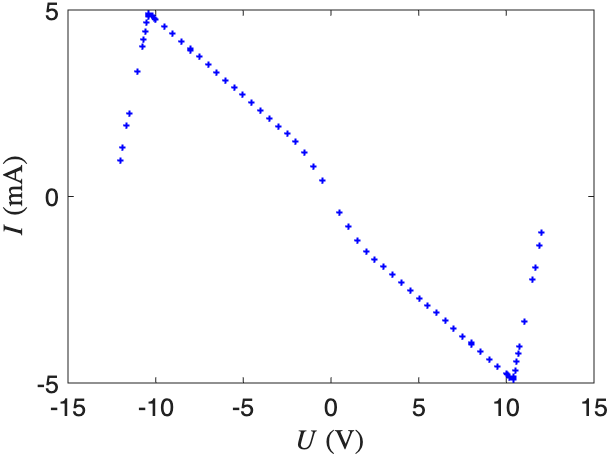
\includegraphics[width=0.6\textwidth]{fig//rn.png} 
                \caption{非线性负阻实验数据散点图}
            \end{figure}

            \begin{figure}
                \centering    
                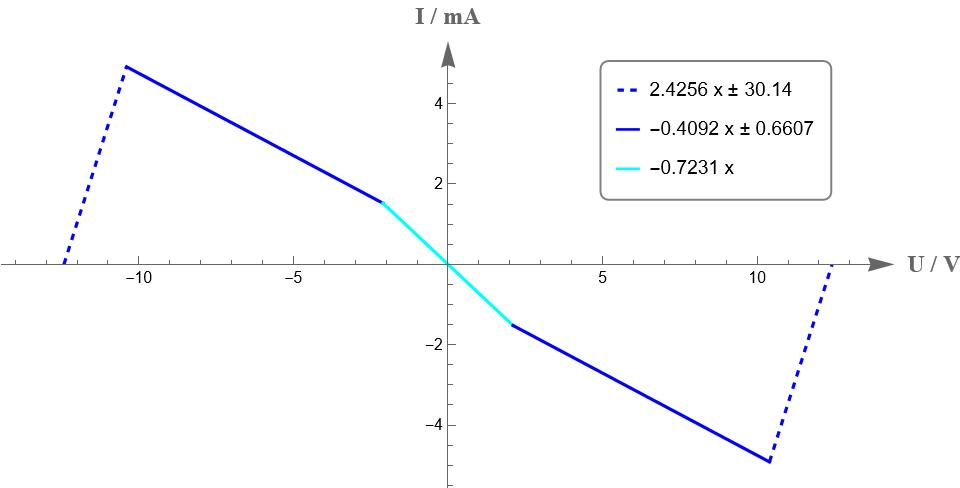
\includegraphics[width=0.6\textwidth]{fig//IUline.jpg} 
                \caption{非线性负阻实验数据拟合图}
            \end{figure}
       
        \subsection{电阻对电路状态的影响}
    
    单调改变蔡氏电路的可变电阻R，在示波器中观察到相图(以C1两端电压为横轴，以C2两端电压为纵轴)发生周期倍分岔式的演化：1P$\to$2P$\to$4P$\to$8P$\to$阵发混沌$\to$3P窗口$\to$单吸引子$\to$不稳定双吸引子$\to$稳定双吸引子。各状态记录如图5所示。
      
        \begin{figure}[h!]
        \centering
        \begin{subfigure}{0.3\textwidth}
            \centering
            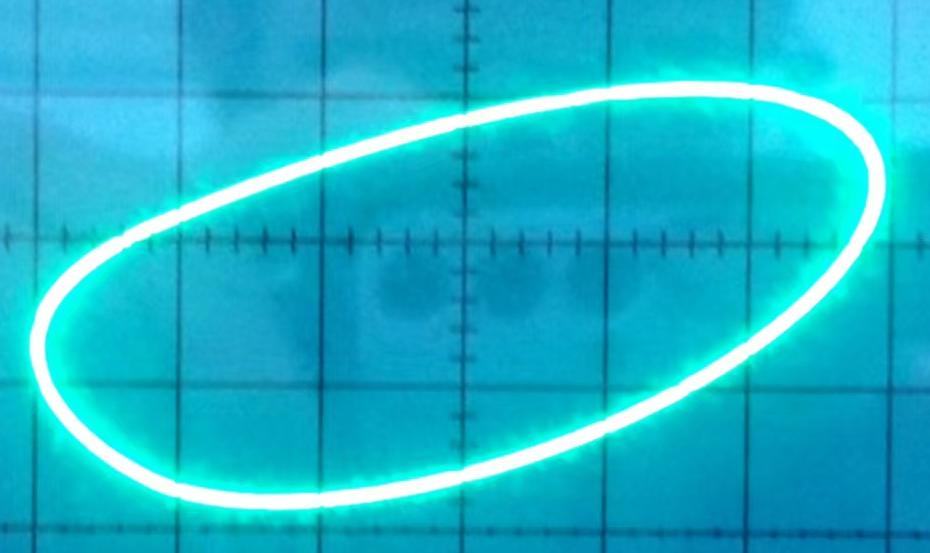
\includegraphics[width=\textwidth,height=\textwidth]{fig//Rmotion//1P}
        \end{subfigure}
        \hfill
        \hspace{5pt}
        \begin{subfigure}{0.3\textwidth}
            \centering
            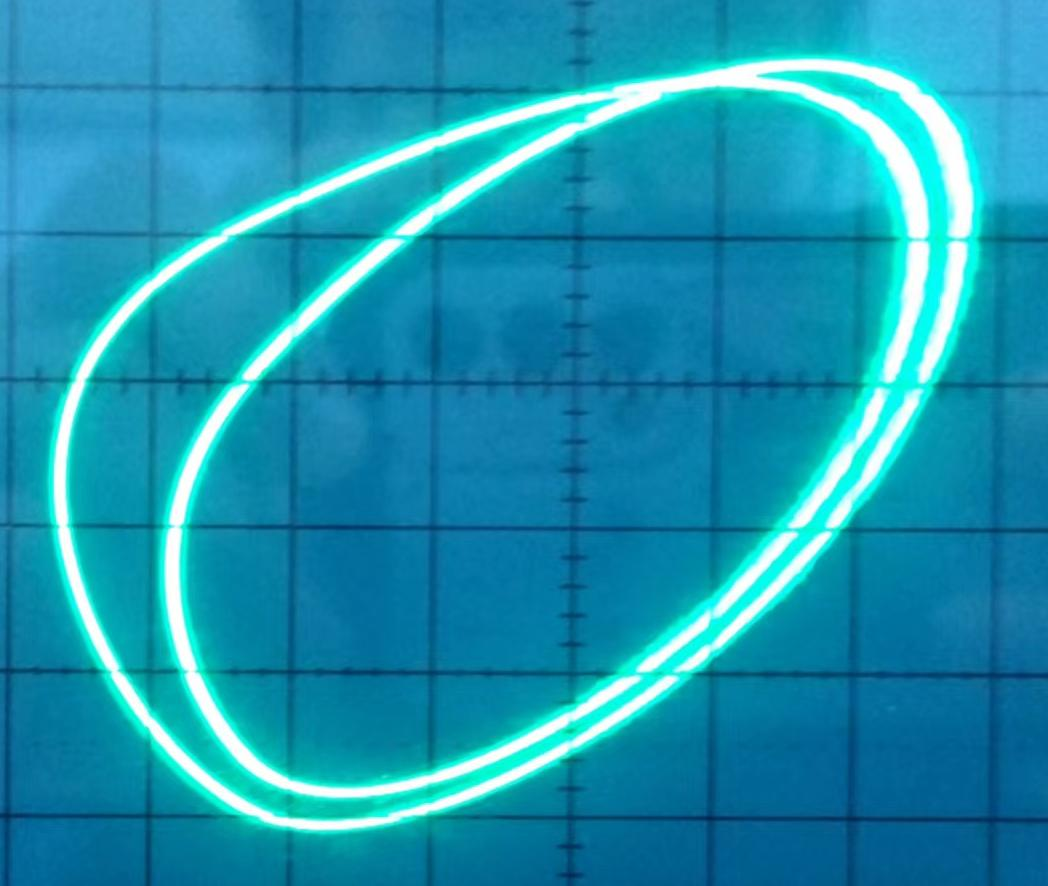
\includegraphics[width=\textwidth,height=\textwidth]{fig//Rmotion//2P}
        \end{subfigure}
        \hfill
        \hspace{5pt}
        \begin{subfigure}{0.3\textwidth}
            \centering
            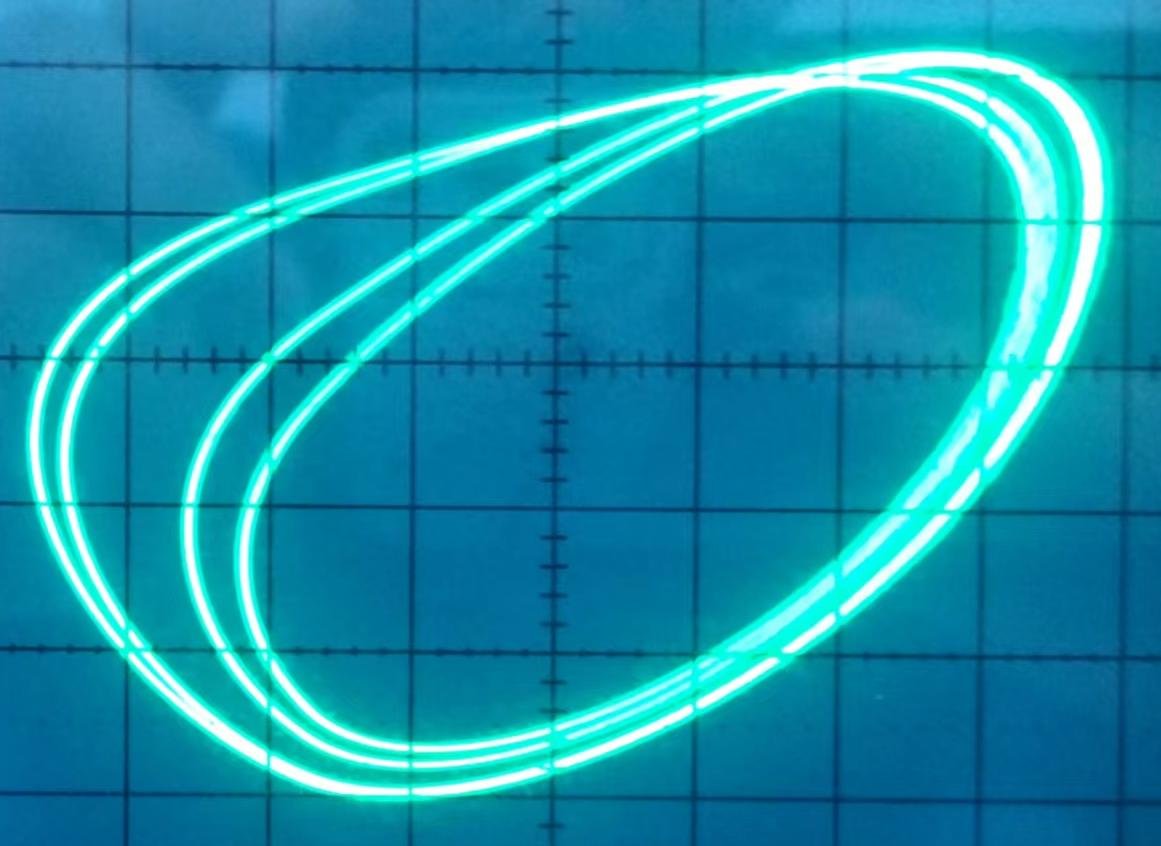
\includegraphics[width=\textwidth,height=\textwidth]{fig//Rmotion//4P}
        \end{subfigure}
        \hfill
        \vspace{5pt}
        \begin{subfigure}{0.3\textwidth}
            \centering
            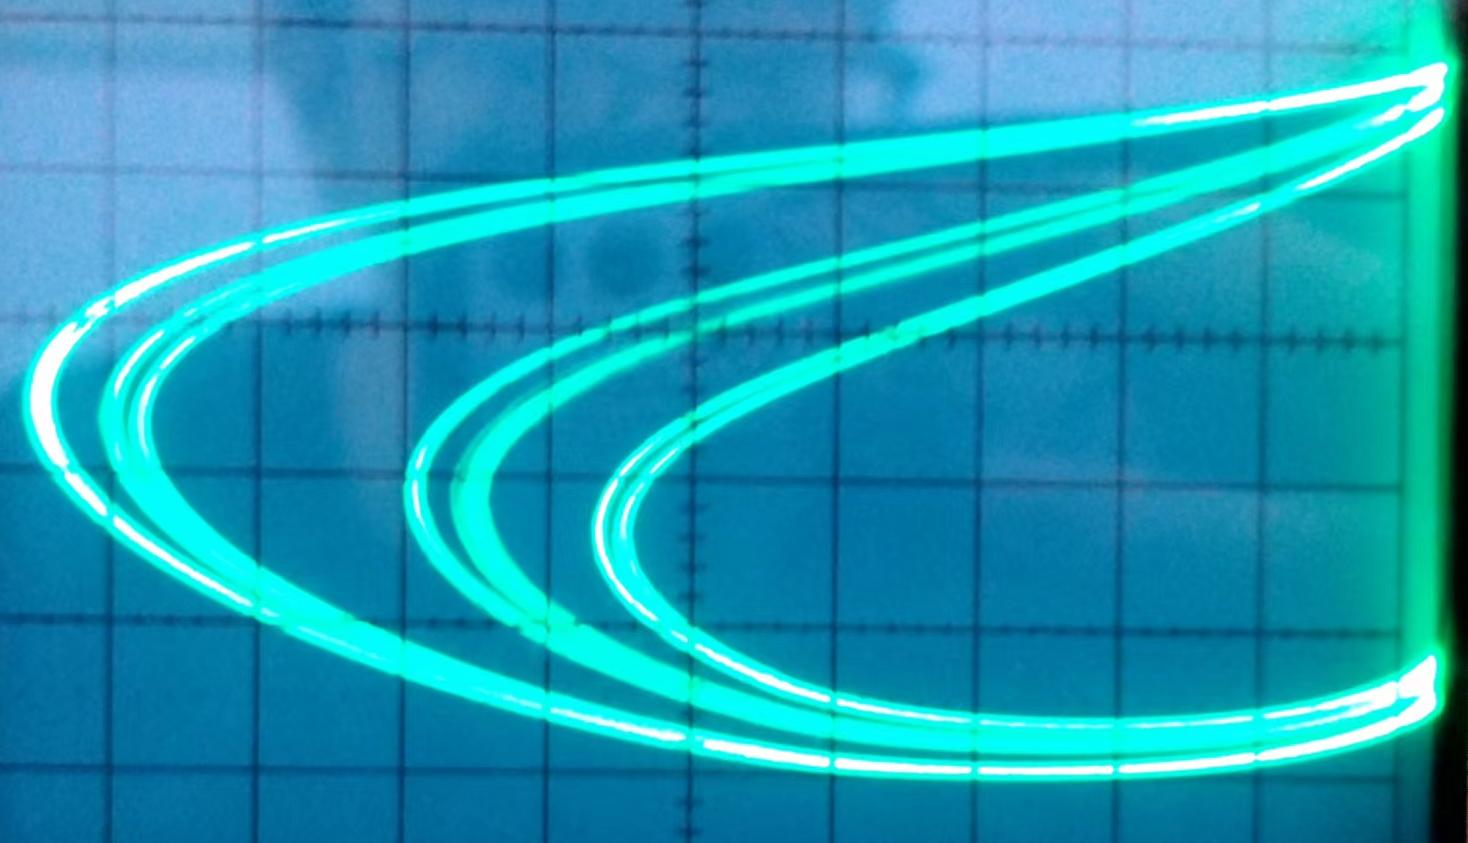
\includegraphics[width=\textwidth,height=\textwidth]{fig//Rmotion//8P}
        \end{subfigure}
        \hfill
        \hspace{5pt}
        \begin{subfigure}{0.3\textwidth}
            \centering
            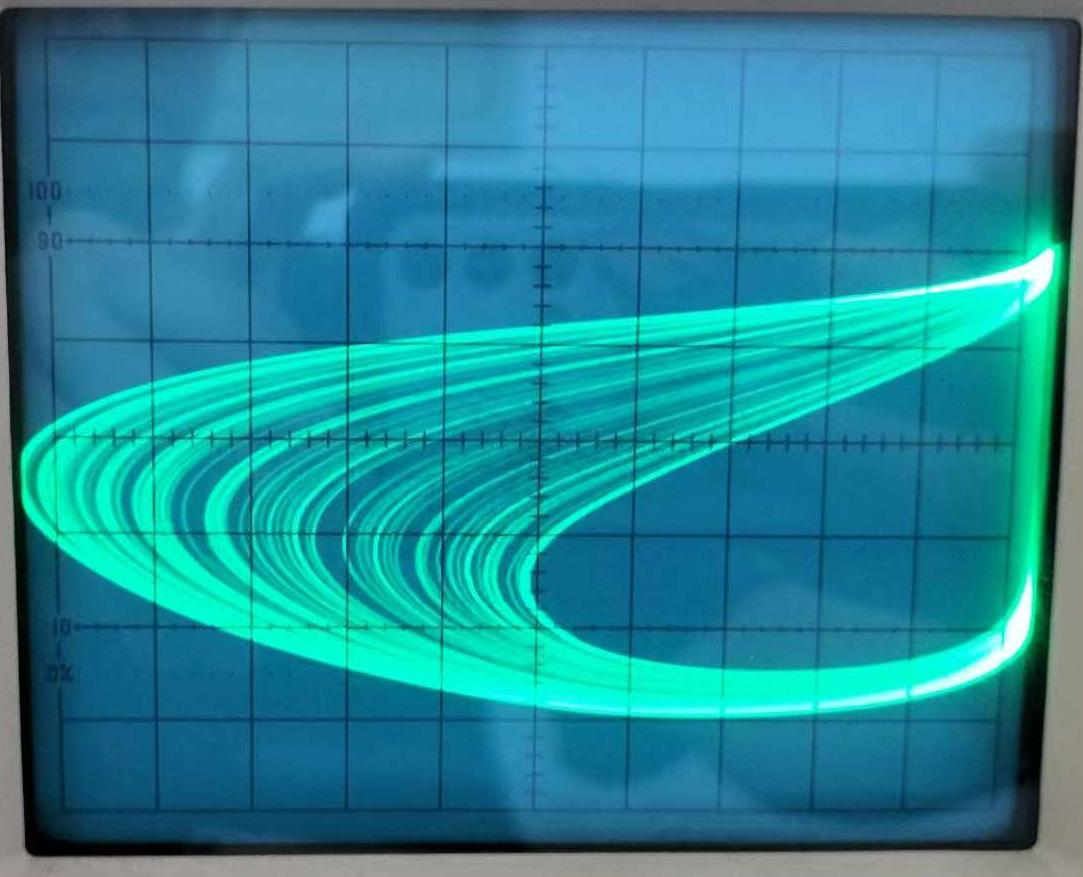
\includegraphics[width=\textwidth,height=\textwidth]{fig//Rmotion//orsochaos}
        \end{subfigure}
        \hfill
        \hspace{5pt}
        \begin{subfigure}{0.3\textwidth}
            \centering
            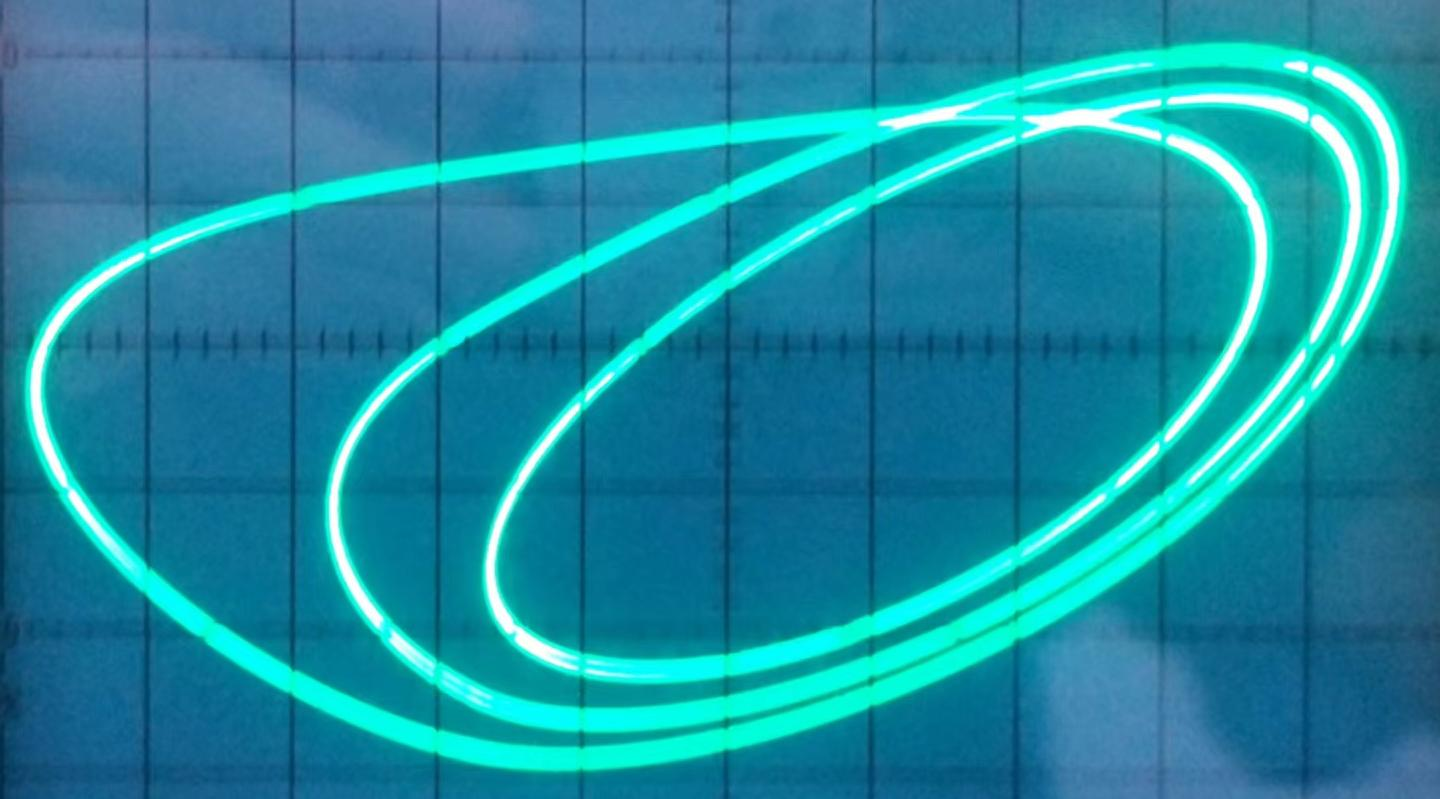
\includegraphics[width=\textwidth,height=\textwidth]{fig//Rmotion//3P}
        \end{subfigure}
        \hfill
        \vspace{5pt}
        \begin{subfigure}{0.3\textwidth}
            \centering
            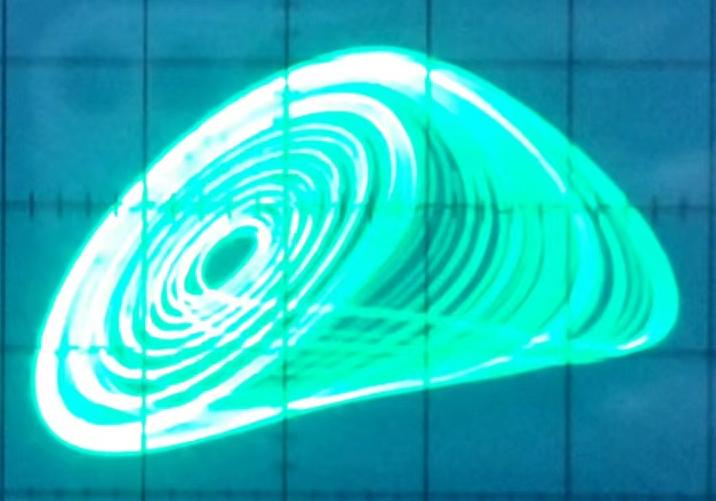
\includegraphics[width=\textwidth,height=\textwidth]{fig//Rmotion//1L}
        \end{subfigure}
        \hfill
        \hspace{5pt}
        \begin{subfigure}{0.3\textwidth}
            \centering
            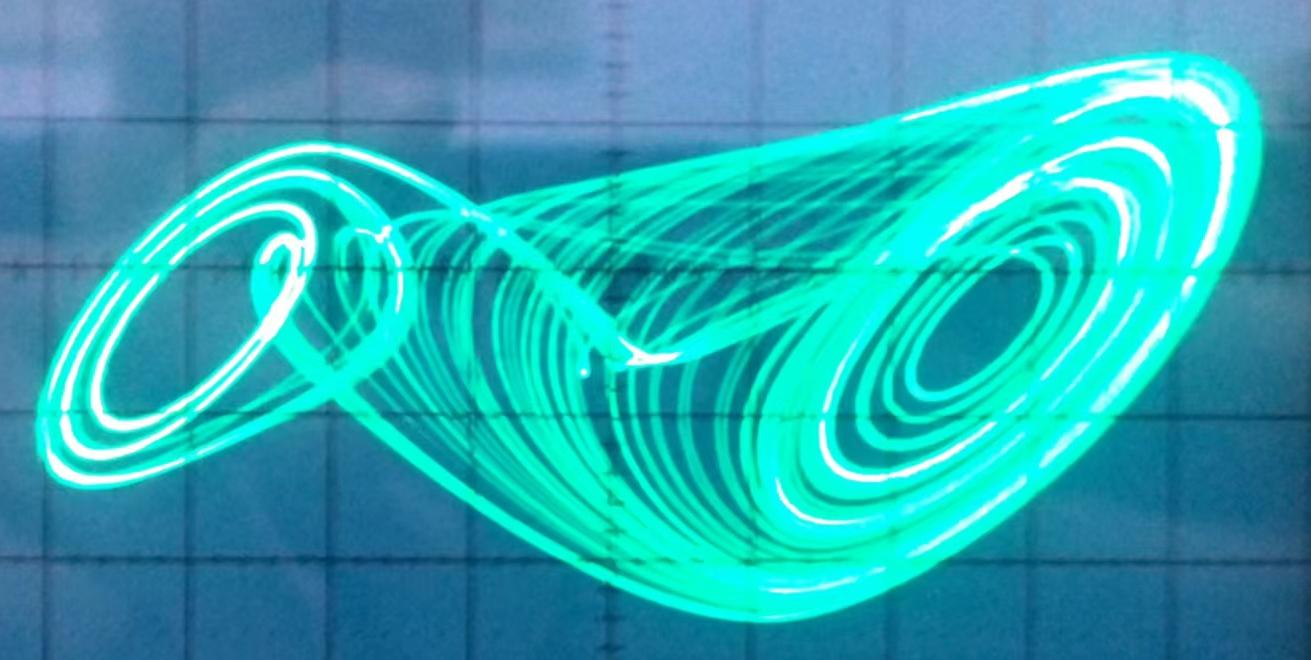
\includegraphics[width=\textwidth,height=\textwidth]{fig//Rmotion//2L1}
        \end{subfigure}
        \hfill
        \hspace{5pt}
        \begin{subfigure}{0.3\textwidth}
            \centering
            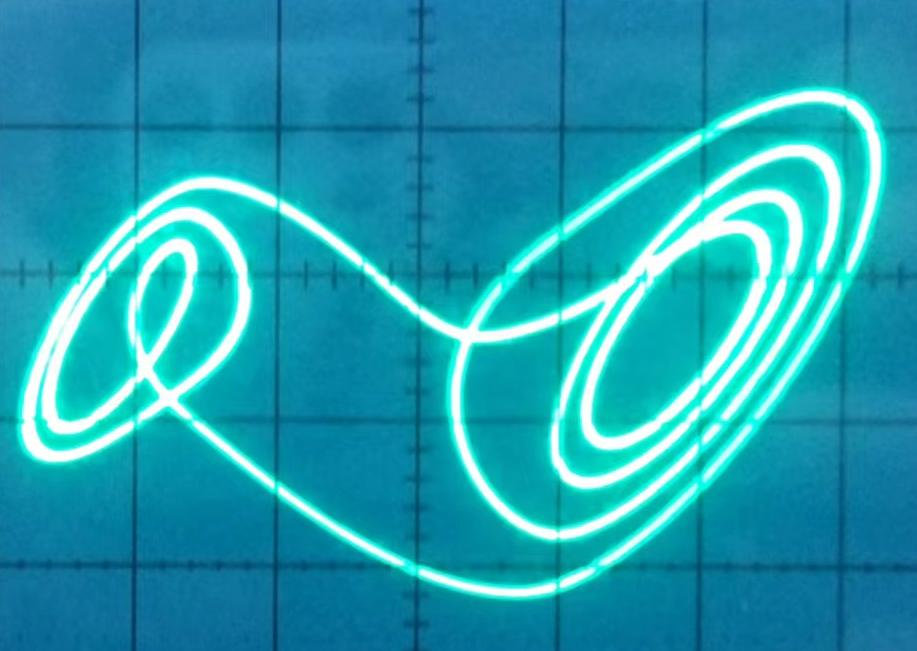
\includegraphics[width=\textwidth,height=\textwidth]{fig//Rmotion//2L2}
        \end{subfigure}
        \vspace{5pt}
        \caption{电路状态的变化}
        \label{fig:Rmotion}
    \end{figure}
     

    \newpage
    \subsection{费根鲍姆常数的测量}

        实验结果如下表1:

        \begin{table}
        \centering
        \caption{费根鲍姆常数的测量}
        \begin{tabular}{ccccc}
            \toprule
            & $2P$ & $4P$ & $8P$ & $\delta$ \\
            \midrule
            \multirow{3}{*}{$C_2/\mathrm{\mu F}$}
            & 0.05487 & 0.05822 & 0.05912 & 3.722 \\
            & 0.06653 & 0.06984 & 0.07075 & 3.637 \\
            & 0.08337 & 0.08662 & 0.08746 & 3.869 \\
            \bottomrule
        \end{tabular}
        \end{table}
     
        \newpage
        实验中测得的费根鲍姆常数明显小于理论值，主要原因可能来自多方面。首先，电路元件（尤其是电容、电阻）存在出厂误差和温度漂移，使得实际的非线性参数与理论模型不符，从而导致分岔点位置偏移。其次，示波器的时间分辨率有限，周期倍化点的判定往往依赖于波形的主观判断，难以精确区分相邻分岔阶段。再次，实验装置中的非理想因素（如放大器的饱和、噪声、器件的迟滞效应等）会使系统偏离理想的逻辑映射模型，使测得的比例系数减小。
    

    \subsection{混沌同步}
        对于搭建的混沌同步电路，在驱动系统和响应系统连接起来之前，首先将两个蔡氏电路处于相同的双吸引子状态，测得两蔡氏电路处于双吸引子状态下的混沌同步和准同步状态如图。
        
        \begin{figure}[h]
    \centering
    % 第一张图
    \begin{subfigure}[b]{0.45\textwidth}
        \centering
        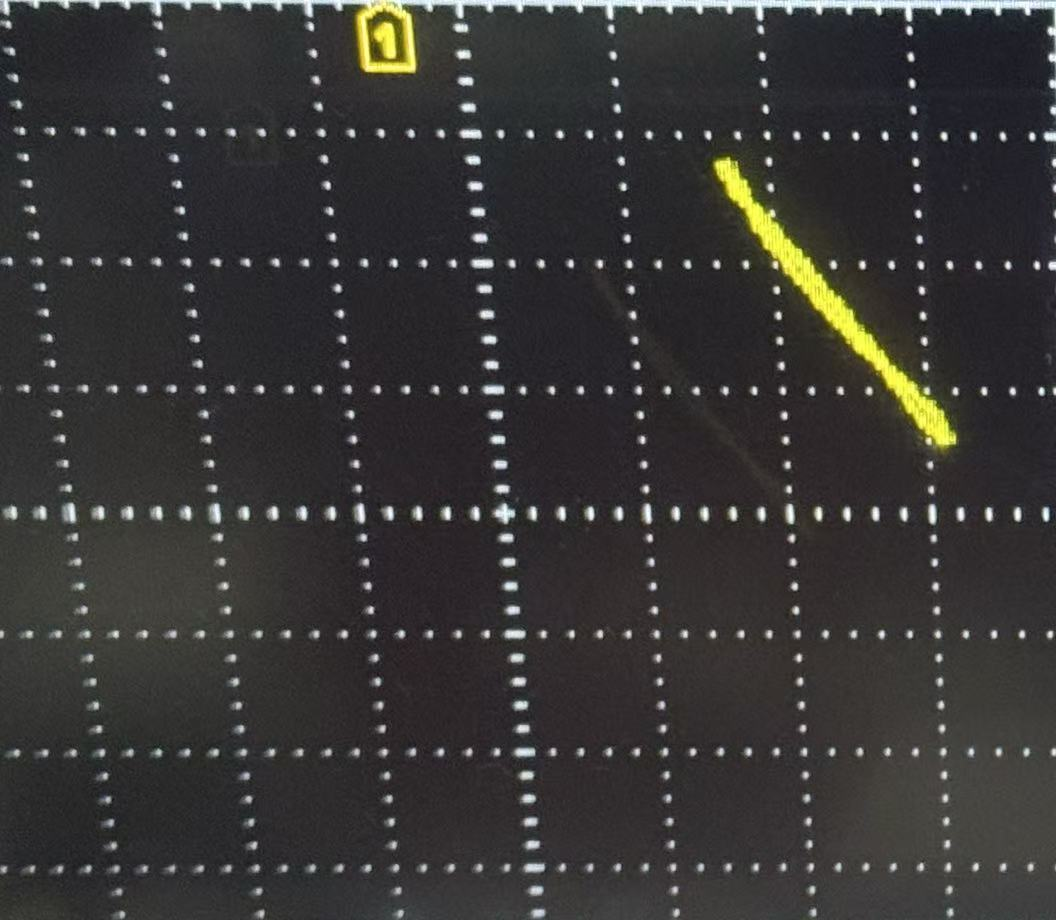
\includegraphics[width=\textwidth]{fig/tb.jpg}
        \caption{同步实验图}
    \end{subfigure}
    \hfill % 在两张图之间自动留空
    % 第二张图
    \begin{subfigure}[b]{0.45\textwidth}
        \centering
        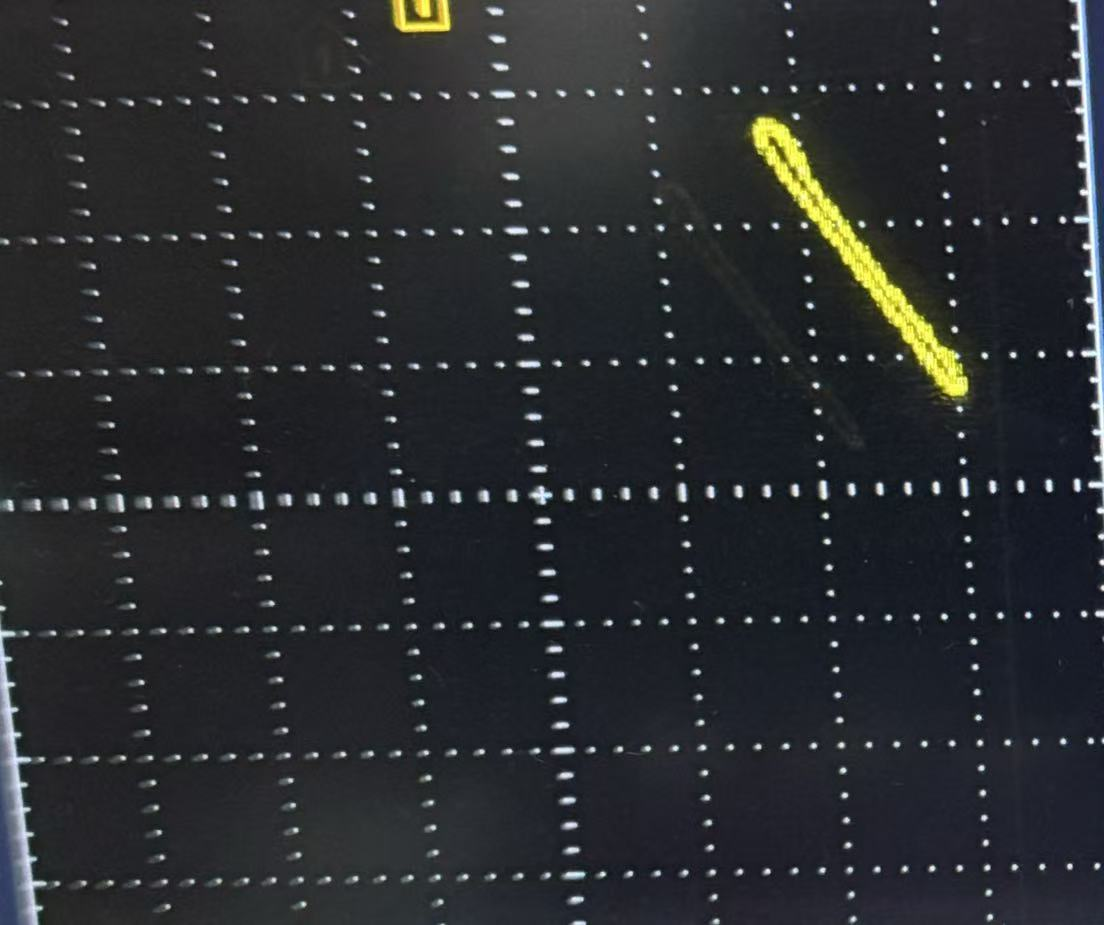
\includegraphics[width=\textwidth]{fig/ztb.jpg}
        \caption{准同步实验图}
    \end{subfigure}
    %
    \caption{同步与准同步实验结果对比}
    \label{fig:sync_compare}
\end{figure}

        \begin{figure}
            \centering    
            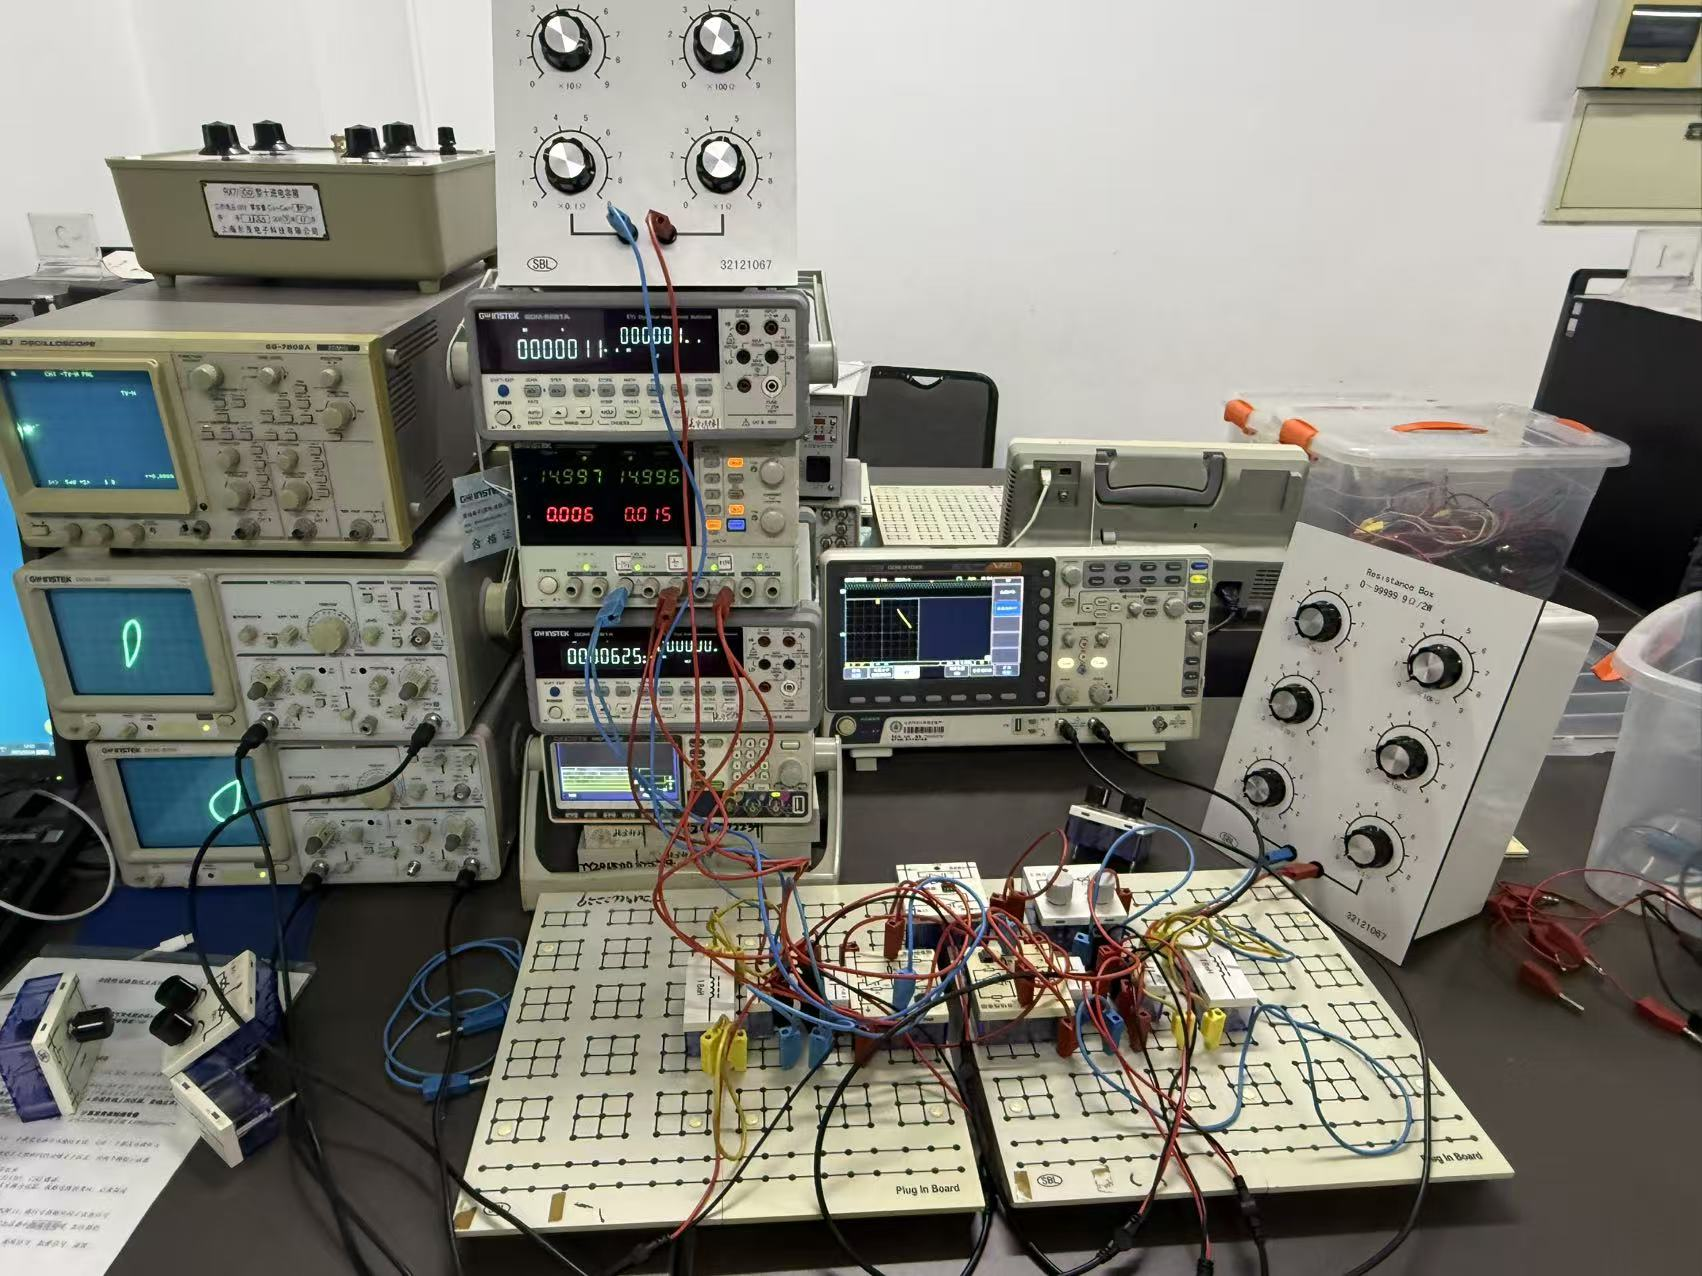
\includegraphics[width=0.9\textwidth]{fig//tbdl.jpg} 
            \caption{混沌同步电路图}
        \end{figure}

        
        
    \newpage
    \subsection{混沌通信}
        将混沌同步电路改造为混动通信电路，向加法器的“混沌信号”端口输入正弦波信号，并在减法器的“混合信号”端口加入驱动系统的混沌信号，将加法器的输出端信号输入到减法器中的“混合信号”端口，记录输入正弦波、混沌信号、加密信号、滤波前信号和滤波后信号。
        
        实验结果如图8所示。
        \begin{figure}
            \centering    
            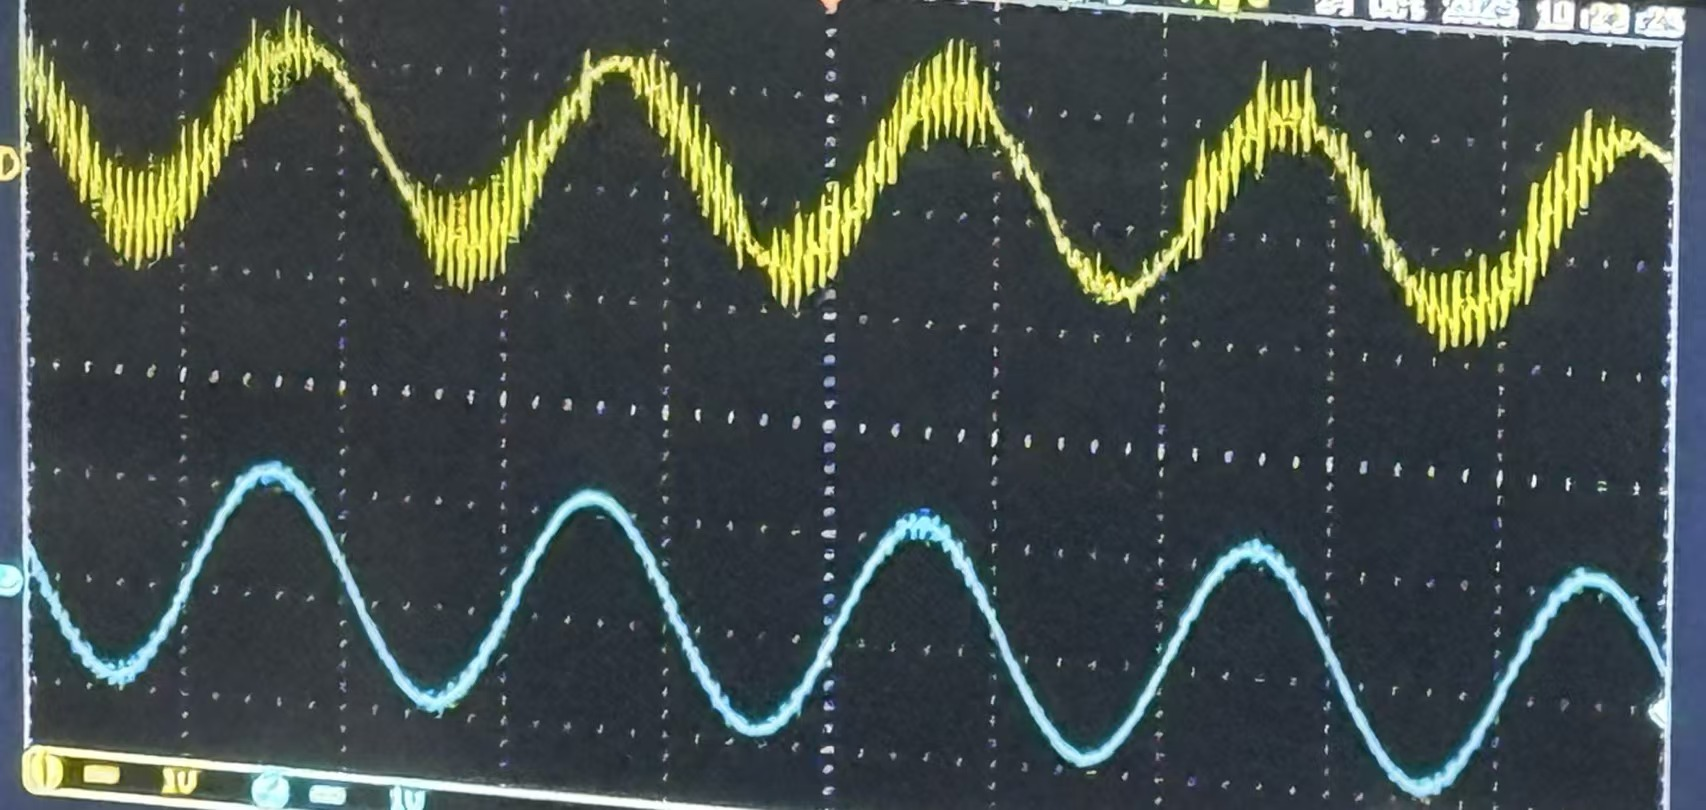
\includegraphics[width=0.8\textwidth]{fig//tx.jpg} 
            \caption{混沌通信电路图(上解密信号，下加密信号)}
        \end{figure}

    \newpage
    \section{总结}
        本实验借助非线性负阻搭建蔡氏电路，完成了与混沌现象有关的一系列实验。我们首先测量了非线性负阻的I-U特性曲线，并得到了负阻不同工作区域的拟合结果：
        
        (1)$I = 2.4256 U + 30.14 $\quad($-12.4258<U<-10.3991$) 
        
        (2)$I = -0.4092 U + 0.6607$\quad($-10.3991<U<-2.10481$)
        
        (3)$I = -0.7231 U $\quad($-2.10481<U<2.10481$)
        
        (4)$I = -0.4092 U + 0.6607$\quad($2.10481<U<10.3991$)
        
        (5)$I = 2.4256 U - 30.14$\quad($10.3991<U<12.4258$) 
        
        （注意上述公式中$I$的单位均为mA，$U$的单位均为V）
        
        接着搭建经典的蔡氏电路探究了电路参数的改变对电路状态的影响，特别地，我们考虑的电阻和电容的影响，分别记录了电路不同动力学状态的周期分岔情况，测量了准费根鲍姆常数$\delta \approx 3.743 $。最后我们借助两个完全相同的蔡氏电路，完成了混沌同步实验和混沌加密通信实验，通过观察电路由同步到准同步的变化，以及记录混沌通信各个过程的信号，加深了对于混沌同步原理和混沌通信原理的认识。

    \begin{thebibliography}{99}
        \bibitem{1}
        北京师范大学物理实验教学中心. 近代物理实验讲义一 (2019)
    \end{thebibliography}

    
\end{document}